% Straight up stealing preamble from Eli Holmes 
%%%%%%%%%%%%%%%%%%%%%%%%%%%%%%%%%%%%%%START PREAMBLE THAT IS THE SAME FOR ALL EXAMPLES
\documentclass{article}

%Required: You must have these
\usepackage{Sweave}
\usepackage{graphicx}
\usepackage{tabularx}
\usepackage{hyperref}
\usepackage{natbib}
\usepackage{gensymb}
\usepackage{authblk}
\renewcommand{\baselinestretch}{1.8}
\usepackage{lineno}
%\usepackage[backend=bibtex]{biblatex}
%Strongly recommended
 %put your figures in one place
 
%you'll want these for pretty captioning
\usepackage[small]{caption}

\setkeys{Gin}{width=0.8\textwidth} %make the figs 50 perc textwidth
\setlength{\captionmargin}{30pt}
\setlength{\abovecaptionskip}{10pt}
\setlength{\belowcaptionskip}{10pt}
% manual for caption http://www.dd.chalmers.se/latex/Docs/PDF/caption.pdf

%Optional: I like to muck with my margins and spacing in ways that LaTeX frowns on
%Here's how to do that
 \topmargin -2cm     
 \oddsidemargin -0.04cm   
 \evensidemargin -0.04cm  % same as oddsidemargin but for left-hand pages
 \textwidth 16.59cm
 \textheight 22.94cm 
 %\pagestyle{empty}       % Uncomment if don't want page numbers
 \parskip 7.2pt           % sets spacing between paragraphs
 %\renewcommand{\baselinestretch}{1.5} 	% Uncomment for 1.5 spacing between lines
\parindent 0pt% sets leading space for paragraphs
\usepackage{setspace}
%\doublespacing

%Optional: I like fancy headers
\usepackage{fancyhdr}
\pagestyle{fancy}
\fancyhead[LO]{How do climate change experiments actually change climate?}
\fancyhead[RO]{2017}
 
%%%%%%%%%%%%%%%%%%%%%%%%%%%%%%%%%%%%%%END PREAMBLE THAT IS THE SAME FOR ALL EXAMPLES

%Start of the document
\begin{document}

% \SweaveOpts{concordance=TRUE}
 \bibliographystyle{/Users/aileneettinger/citations/Bibtex/styles/amnat.bst}
\setkeys{Gin}{width=\textwidth}
\title{How do climate change experiments actually change climate?} 
\author[1,2,*]{A.K. Ettinger}
\author[3]{I. Chuine}
\author[4,5]{B.I. Cook}
\author[6]{J.S. Dukes}
\author[7]{A.M. Ellison}
\author[8]{M.R. Johnston}
\author[9]{A.M. Panetta}
\author[10]{C.R. Rollinson}
\author[11,12]{Y. Vitasse}
\author[1,8]{E.M. Wolkovich}
\affil[1]{Arnold Arboretum of Harvard University, Boston, Massachusetts 02131, USA}
\affil[2]{Tufts University, Medford, Massachusetts 02155, USA}
\affil[3]{CEFE UMR 5175, CNRS, Universit\'e de Montpellier,Universit\'e Paul-Val\'ery Montpellier, EPHE, Montpellier, France}
\affil[4]{Lamont-Doherty Earth Observatory, Columbia University, Palisades, New York 10964, USA}
\affil[5]{NASA Goddard Institute for Space Studies, New York, New York 10025, USA}
\affil[6]{Department of Forestry and Natural Resources
and Department of Biological Sciences, Purdue University, West Lafayette, Indiana 47907, USA}
\affil[7]{Harvard Forest, Harvard University, Petersham, Massachusetts 01366, USA}
\affil[8]{Department of Organismic and Evolutionary Biology, Harvard University, Cambridge, Massachusetts 02138, USA}
\affil[9]{Department of Ecology and Evolutionary Biology, University of Colorado, Boulder, Colorado 80309, USA}
\affil[10]{The Morton Arboretum, Lisle, Illinois 60532, USA}
\affil[11]{Institute of Geography, University of Neuch\^atel, Neuch\^atel, Switzerland}
\affil[12]{Swiss Federal Institute for Forest, Snow and Landscape Research WSL, Neuch\^atel, Switzerland}
\affil[*]{Corresponding author: aettinger@fas.harvard.edu}
%\date{\today}
\maketitle  %put the fancy title on
%\tableofcontents      %add a table of contents
%\clearpage
%%%%%%%%%%%%%%%%%%%%%%%%%%%%%%%%%%%%%%%%%%%%%%%%%%%
%We argue that it is critical for scientists to better understand and report climate from climate change experiments.
%Ben's suggestion: *I just have an overall general comment on the framing of the paper. I think it’s great and would be happy to see it published more or less as is. However, you might consider some rewriting or reorganizing around the two QUESTIONS that I think this paper really gets at:
%	-Did the experimental warming increase the temperature has much as it was supposed to? If not, how off were the treatments from the target warming and why?
%	-What other climate variables (e.g., soil moisture) or statistics (e.g., variability, extremes) change along with the warming treatment?
%Such a reorganization might just make the paper a little more readable and compelling, and give an even firmer narrative hook for the reader to latch onto. Anyway, just my two cents! 

%Main things to address based on NCC reviews:
%i.	Justify our use of experiments only more…
%1.	Don’t mention precip in the beginning. 
%2.	Get maximum variability/amount in temperature
%3.	Passive warming doesn’t warm as much 
%4.	Say how many datasets looked at
%5.	Say who declined in supplement
%6.	Change the wording
%7.	Two or three full sentences on why we’re not looking at passive warming. We do not include passive worming because they have the following problems (that are generally unique to OTCs). OTCs have to be analyzed on their own. Set of issues that apply mostly to them.
%ii.	Include models/figure for phenology? Then suggest that we need to study how widespread this is.
%iii.	Minor things:
%1.	Improve legends, explain some points more.

\linenumbers

\section* {Preface} 
\par To understand and forecast biological effects of climate change, scientists frequently use field experiments that alter temperature and precipitation (e.g., with infrared heaters, rain shields, and supplemental watering). These experimental results may be interpreted in misleading ways, however. Using a new database of daily climate data from 12 active warming experiments, we find that the common practice of summarizing and analyzing only the mean changes across treatments hides potentially important variation in treatment effects over space and time. Furthermore, treatments produce unintended secondary effects, such as soil drying in conjunction with warming. The implications of these complexities are rarely explored, but have important biological consequences. We show one example of such consequences with a case study of spring plant phenology, in which such secondary effects lead to inaccurate quantification of species' sensitivities to changes in temperature. Based on our findings, we present several recommendations for future experimental design, analysis, and data sharing that we believe will improve the ability of climate change experiments to accurately identify and forecast species' responses.
\section* {Introduction}
\par Climate change is dramatically altering earth's biota, shifting the physiology, distribution, and abundance of organisms, with cascading community, ecosystem, and climate effects \citep{shukla1982,cox2000,thomas2004,parmesan2006,field2007,sheldon2011,urban2012}. Much uncertainty exists about how particular individuals, populations, species, communities, and ecosystems will respond as shifts in temperature and precipitation regimes become more extreme. Predicting biological responses to current and future climate change---and how they will feedback to affect earth's climate and ecosystem services---are among the most significant challenges facing scientists today.

\par Two common approaches for understanding biological effects of climate change are observational studies and process-based modeling; yet these approaches are insufficient for several reasons. Observational studies, which correlate recorded biological patterns with measured trends in climate, cannot disentangle the causal effects of warming from other factors that have also changed over time, such as successional stage or land use. Process-based models can overcome some of these challenges because they rely on explicit empirical relationships between observed phenomena and climate. They, however, are limited by their underlying assumptions, which may be poorly constrained \citep [e.g.,][]{pearson2004,ibanez2006,swab2012,chuine2016}. In addition, neither approach is well-vetted for predicting future conditions that fall outside the range of historical variability; climate change will yield warmer temperatures than the previous 150 years, and possibly warmer than at any time in the last 2000 years \citep{ohlemuller2006,williams2007,williams2007b,ipcc2013}.  

\par Field-based experiments that alter temperature address these shortcomings, and are therefore critical for determining mechanistic links between climate change and biological responses \citep[e.g.,][]{box1978,williams2007,gelman2014}. Experiments can quantify biological responses to different levels of climate change, and can create the ``no-analog" climate scenarios forecasted for the future, particularly when they employ active warming methods, such as gas-powered forced air heaters, electrical-powered soil warming cables, or infrared heaters \citep{shaver2000,williams2007b,aronson2009}. In addition, active warming can be combined with precipitation manipulations (e.g., snow removal, water additions, water reductions), offering the ability to isolate effects of temperature and precipitation from other environmental changes \citep [e.g.,][]{price1998,cleland2006,sherry2007,rollinson2012}. %Furthermore, if regression designs are used \citep[e.g.,][]{pelini2011} and a range of warming and precipitation treatments are applied, non-linear responses can be estimated. 
Compared with indoor growth-chamber experiments, field-based experiments offer the possibility of preserving important, but unknown or unquantified feedbacks among biotic and abiotic components of the studied systems. 

\par Climate experiments allow ecologists to draw conclusions about how climate change may affect species' growth, survival, and future distributions \citep{dukes1999,hobbie1999,morin2010,chuine2012,reich2015,gruner2016}. But is it reasonable to extrapolate findings from these experiments to the real world? Do they actually alter climate in the ways that we think they do? Recent research suggests that climate manipulations do not alter climate in ways that are consistent with observed changes over time \citep{wolkovich2012,menke2014}. However, we lack a robust assessment of how active warming experiments alter the climate conditions experienced by organisms, and the extent to which these conditions are similar to current field conditions or anticipated climate change. 

\par Here, we investigate if and how climate change experiments actually change climate. Using plot-level daily microclimate data from 12 active warming experiments (yielding 41 experiment years) we show the direct and indirect ways that experimental manipulations alter climate. We highlight the challenges associated with quantifying and interpreting experimental shifts in climate and the resulting biological responses. Finally, we use findings from our synthesis to make recommendations for future climate change experiments (Box 1). We focus on \textit{in situ} active warming manipulations, because recent analyses indicate that active warming methods are the most controlled and consistent \citep{kimball2005,kimball2008,aronson2009,wolkovich2012}. The data we use were collected between 1991 and 2014 from North American and European climate change experiments (Figure \ref{fig:map}, Tables S1, S2) and have been merged into a new, publicly available Climate from Climate Change Experiments (C3E) database \citep{ettinger2017}. 

\section* {Complexities in interpreting experimental climate change} 

Climate change experiments often include detailed monitoring of climate variables at the plot level, yielding large amounts of data, such as daily or hourly temperature and other climate variables, over the course of the experiment. Biologists, however, are generally interested in the biological responses (e.g., community dynamics, species' growth, abundance, or phenology), which are collected on much coarser timescales (e.g., weekly or annually). Not surprisingly, then, authors typically provide detailed information on the observed biological responses, but report only the mean change in climate over the course of the experiment and whether it matched their target level of change \citep[e.g.,][]{price1998,rollinson2012,clark2014a,clark2014b}. 

% This next paragraph is critical -- be sure to include jist of it in cover letter (and consider moving up if we ever change formatting of paper). This contains the main point of the paper. could leave as is
\par Though the published focus is often on shifts in mean climate variables, imposed climate manipulations actually result in much more complex shifts. The magnitude of change in these manipulations may vary in time and space, and the presence of experimental equipment often unintentionally alters environmental conditions. These factors, discussed below, challenge our interpretation of how experimental warming studies can be used to forecast effects of climate change.

\subsection* {Effects on local climate vary over time and space}
Reporting only the mean temperature difference across the duration of the study hides potentially important variations in daily, seasonal, and annual temperatures among treatments. Using the C3E database, we found that active warming reduces above-ground daily temperature range (DTR) (Table S3, see also Table S2, which details the different methods used to measure temperature). Active warming decreased above-ground DTR by differentially affecting maximum and minimum temperatures: warming increased daily minima by 0.84\degree C per \degree C of warming target, but only increased daily maxima by 0.51\degree C per \degree C of target warming (Tables S3). %This may be similar to what is projected for parts of the world, since DTRs are expected to change; however, shifts in the DTR will likely vary spatially, as some regions have experienced greater daytime warming than nighttime warming, whereas others have experienced the opposite \citep{ipcc2013}. 
%AM: This last sentence doesn’t add much because it is vague.  How about replacing it with a statement about how soil DTRs changed?

\par We observed strong seasonal and annual variations in experimental warming effects (Figures \ref{fig:effwarm}, \ref{fig:blockyear}, Table S4). These may be driven by interactions between warming treatments and daily, seasonal, and annual weather patterns, since the magnitude of warming may vary as weather conditions change.  Both infrared heaters and soil cables fail to achieve the target temperatures during rainstorms \citep{peterjohn1993,hoeppner2012} and with windy conditions \citep{kimball2005,kimball2008}. In addition, treatments are often applied inconsistently within or across years. Heat applications are frequently shut off during winter months, and some heating methods, even if left on throughout the year, are not capable of applying constant warming year-round \citep[e.g.][]{clark2014a,clark2014b,hagedorn2010}. 

\par Treatment effects also vary spatially, adding further complication to interpreting effects of climate change experiments. The C3E database contains four studies that used blocked designs, allowing us to examine spatial variation in the amount of warming (i.e. the difference between treatment and control plots within a block). We found that the amount of observed warming varied significantly by more than 1\degree C among blocks (Figure \ref{fig:blockyear}, Table S5); block-to-block variation in warming treatment varied by 60-100\% of target temperatures. These differences in warming levels among blocks may be caused by fine-scale variation in vegetation, slope, aspect, soil type, or other factors that can alter wind or soil moisture, which in turn affect warming \citep{peterjohn1993,kimball2005,kimball2008,hoeppner2012,rollinson2015}. 

\par Of course, identical experimental treatments across space and time are not necessary for robust analysis of experimental results or for forecasting. Indeed, the spatial and temporal variation we report could improve and refine models, and---at least in some regions---may be consistent with contemporary patterns of climate change \citep{ipcc2013}. Taking advantage of this variation, however, requires understanding and reporting it \citep[e.g.,][]{milcu2016}. In contrast, fine-scale spatial and temporal variations in warming treatments are rarely analyzed explicitly, so the implications for interpretation of experimental findings are unclear.

\subsection* {Experimental infrastructure alters local climate}
Experimental structures themselves can alter temperature and other important biotic and abiotic variables in ways that are not generally examined nor reported in experimental climate change studies. The importance of controls that mimic a treatment procedure without actually applying the treatment is widely acknowledged in biology \citep[e.g.,][]{spector2001,johnson2002,quinn2002}. Though some researchers install treatments with non-functional warming equipment in experimental climate change studies, the magnitude and implications of structural effects on climate are rarely discussed or interpreted.
\par To investigate the magnitude of infrastructure effects, we compared temperature and soil moisture data from five active warming studies at two sites: Duke Forest and Harvard Forest \citep{farnsworth1995,clark2014b, marchin2015, pelini2011}. These were the only studies in the C3E database that monitored climate in two types of control plots: structural controls (i.e., `shams' or `disturbance controls,' which contained all the warming infrastructure, such as soil cables or infrared heating units but with no heat applied) and ambient controls with no infrastructure added. Other studies monitored environmental conditions in only structural controls (n=3) or only ambient controls (n=4).

\par We found that experimental structures altered above-ground and soil temperatures in opposing ways: above-ground temperatures were higher in the structural controls than in ambient controls, whereas soil temperatures were lower in structural controls compared with ambient controls (Figure \ref{fig:shamamb}a-d). This general pattern was consistent across different temperature models (mean, minimum, and maximum temperatures), although the magnitude varied among seasons, studies, and years (Figure \ref{fig:shamamb}a-d, Tables S6-S11). We also found that experimental infrastructure decreased soil moisture relative to ambient conditions (Figure \ref{fig:shamamb}e, Tables S8, S11). 

\par There are several possible reasons for the observed climatic differences between ambient and structural controls. Infrastructure materials may shade the plots, reduce airflow, reduce albedo relative to surroundings, or otherwise change the energy balance. Structures also interfere with snow accumulation, thereby reducing snowpack and its insulation. %AE: Is it worth noting that passive warming experiments (e.g., ITEX or other open plastic greenhouses) illustrate clearly that the infrastructure by itself alters the climate? An ITEX chamber = a "sham" control in a warming experiment!
This likely plays a bigger role in soil temperature differences at the Harvard Forest sites (exp04, exp07, exp08), where average annual snowfall is over one meter, than at Duke Forest (exp03,exp10), where average snow accumulation each winter is 20 cm or less. Although there is little discussion of measured temperature (or other) differences between ambient and structural control plots in published work \citep[e.g.,][]{farnsworth1995,pelini2011,clark2014a,clark2014b}, Clark \textit{et al.} (2014b) mention that ``control of the air temperature was less precise, in part due to air scooping on windy days." Marchin \textit{et al.} (2015) note that structural controls had mean spring air temperatures about  0.5\degree C or more above ambient temperatures and Peterjohn \textit{et al.} (1994) reported cooler soil temperatures in structural controls than in ambient controls at shallow soil depths. Similarly, we found the greatest difference in soil temperature between structural and ambient controls in shallow soils (e.g. exp10, soil depth = 2cm). Further, while the focus to date has been largely on these abiotic impacts of experimental structures, such structures may also alter herbivory and other biotic conditions \citep{kennedy1995,moise2010,wolkovich2012,hoeppner2012}. 

\par Most warming experiments calculate focal response variables relative to ambient controls \citep [e.g.,][]{marchin2015}, which our analyses suggest will not properly account for infrastructure effects. Because the design of these experiments may influence abiotic and biotic responses in warming experiments, improved documentation and analysis of infrastructure effects is an important next step in climate change experiments, particularly if we wish to apply results to forecasting.

\section* {Secondary and feedback effects of climate change manipulations} 
Climate change experiments often seek to manipulate one or two climate variables, usually temperature and precipitation, but manipulating either of these variables also alters the other. Precipitation treatments typically reduce temperatures in climate change manipulations \citep{sherry2007,rollinson2012,mcdaniel2014}: McDaniel et al. (2014) observed that a twenty percent increase in precipitation reduced mean hourly temperatures by 0.3\degree C over the course of their two-year experiment. Experimental warming typically increases vapor pressure deficit and reduces soil water content \citep[e.g.,][]{sherry2007,morin2010,pelini2014,templer2016}. Of the twelve experiments in the C3E database, we examined the ten that measured and reported soil moisture and found that experimental warming reduced soil moisture by 3.0\%, on average (Figure 5, Table S13), and that this reduction occurred at a rate of 0.43\% per degree of target warming (Table S12). Thus, although active warming experiments may not be explicitly designed to manipulate soil moisture, soil moisture is unavoidably affected by changing temperatures. 

\par Warming and precipitation treatments, and their secondary effects on soil moisture and other abiotic factors, can also alter the biotic environment, which may produce cascading effects. Many studies have found shifts from herbaceous to woody plant communities with experimental warming \citep[e.g.,][]{rollinson2012, mcdaniel2014,mcdaniel2014b, harte2015}; this, in turn, can alter microbial and herbaceous plant communities. These community shifts may change competitive dynamics and affect resource levels, such as moisture, carbon, and nutrients in the soil \citep{mcdaniel2014,mcdaniel2014b, harte2015}, and cause positive feedbacks to local climate change \citep{harte2015}. 

\par The widespread presence of unintended secondary effects of climate change manipulations highlights the importance of measuring environmental conditions at the plot level, and using these measurements in analysis and interpretation of results. Many climate change experiments---including seven of the 12 in the C3E database---analyze warming and/or precipitation treatments as simple categorical predictors (e.g., as in a two-way ANOVA). Our findings, however, demonstrate a clear need for alternative modelling approaches to fully understand the experimental results and to make mechanistic links between changes in climate and ecological responses. One straightforward alternative is to include the continuous climate data (e.g., plot-level mean temperatures) as predictors of the focal response variable, such as phenological state or species density \citep [e.g.,][]{marchin2015, pelini2014}. 
%Find a new place for this point/citation: A challenge with this approach is that much of the true variation in the climate is lost through aggregation (e.g., calculating mean annual or seasonal temperature), and the chosen method of aggregation affects both the mean and variance of the climate estimate \citep [e.g.,][]{clark2014b}. 

\section* {Biological implications}

\par We have highlighted a suite of factors that complicate interpretation of warming experiments. These largely unintended alterations are likely to have biological implications for many of the major responses studied in warming experiments (e.g., Figure \ref{fig:biolimp}). Interpretation of experimental climate change effects on biological responses may be misleading, because the intended climate treatments (i.e., categorical comparisons or target warming levels) are generally used as explanatory variables in analyses. The interpretation is likely to be altered by using fine-scale, measured climate as explanatory variables. Detailed examination of multiple microclimate variables (e.g., plot-level temperature and soil moisture) will allow a more complete understanding of the indirect, as well as direct, effects of treatments on abiotic and biotic drivers of focal responses.

\par Plant phenology provides one example of a biological response that is muted in experiments versus observational studies (Figure \ref{fig:biolimp}b). This is because phenology has a complex dependence on temperature and water availability (as well as other factors). Although phenology is generally advanced by higher spring temperatures, it can also be delayed by increased winter temperature (which delays endodormancy break). In addition, reduced water availability during the spring can slow cell elongation and delay budburst \citep{penuelas2004,ourcival2011,craine2012,matthews2016}.

Effects of these different drivers may be responsible for the observed discrepancy between observational and experimental phenological responses to warming \citep{wolkovich2012}. Other biological responses may be exaggerated in experiments when direct and indirect effects of climate manipulations work in concert (Figure \ref{fig:biolimp}c). Accounting for both direct and indirect effects of warming is critical for accurate interpretation of the consequences of climate change \citep{kharouba2015}. Since climate change experiments have indirect effects on the biotic as well as abiotic environment \citep{hoeppner2012,pelini2014,diamond2016}, a critical question is the extent to which these indirect effects are accurate forecasts of future shifts that are likely to occur with climate change, or due to side-effects that are unlikely to occur outside of experimental systems \citep{moise2010,diamond2013}.
\section* {Conclusions}
\par As climate change continues across the globe, ecologists are challenged to not only document impacts but make quantitative, robust predictions. Our ability to meet this challenge requires a nuanced mechanistic understanding of how climate directly and indirectly alters biological processes. Climate change experiments, which have been underway for nearly four decades \citep[e.g.,][]{tamaki1981,carlson1982}, provide invaluable information about biological responses to climate change. Yet the full range of changes in environmental conditions imposed by these experiments is rarely presented. We have compiled the first database of fine-scale climate data from multiple warming experiments and shown how time, space, and experimental artifacts may hinder simple interpretations of these climate change experiments. We hope this provides a foundation for gaining the most knowledge and utility from existing experiments, for designing better experiments and models in the future (see Box 1), and for improved understanding of biological responses and feedbacks in a changing world
 \section* {Acknowledgements}
We are grateful to those who shared their experimental climate data with us and others in the C3E database. We thank the Radcliffe Institute for Advanced Study at Harvard University, which provided funding for an Exploratory Seminar at which the ideas in this paper were conceived. This research was also supported by the National Science Foundation (NSF DBI 14-01854 to A.E.). Any opinion, findings, and conclusions or recommendations expressed in this material are those of the authors and do not necessarily reflect the views of the National Science Foundation.
\section*{Data Accessibility}
The C3E database will be available at KNB \citep{ettinger2017}, along with all R code from the analyses included in this paper. (Currently, metadata is published there; the full database and R code are available to reviewers upon request.)

\section*{Author contributions} All authors conceived of this manuscript, which was inspired by our discussions at a Radcliffe Exploratory Seminar in 2016, and all authors edited the manuscript. A.E. and E.W. conceived of the idea for the database and related Radcliffe Exploratory Seminar. A.E. compiled the datasets; A.E. and C.R. analyzed the data and created the figures; A.E. wrote the manuscript.

\section* {Box 1: Recommendations for future climate change experiments} 
\begin{enumerate}
\item\textit{Collect and analyze fine-scale climate data.} This includes analyzing and interpreting minimum and maximum values, as well as variance and critical thresholds \citep[e.g., the number and duration of freeze-thaw events and accumulated chilling hours,][]{mcdaniel2014,vasseur2014}. We suggest saving the raw data from data loggers (often collected at hourly or higher resolution) to allow quantification of variance (and other summaries) at different temporal resolutions. In assessing which frequency of measurements is most appropriate for analyses (e.g., hourly, twice daily), it is critical to consider the chronobiology of the event and organisms of interest. For ants, this might mean that temperatures be monitored every minute \citep{shavit2017}; for bacteria, even more frequently. 
\item\textit{Analyze measured climate variables rather than targets}. There can be substantial variation in the effects of warming and precipitation treatments among plots and across time (Figure \ref{fig:blockyear}). Analyzing measured climate will allow much more in-depth understanding of the drivers and biological effects of variation in temperature and moisture.
\item\textit{Publish high quality, usable data and metadata}. Given that in situ active climate manipulations are logistically challenging and expensive \citep{aronson2009}, and that they often produce a large volume of fine-scale climate data, good curation and data sharing will ensure wider use and deeper understanding of these valuable data. When studying biological implications of a global challenge as large as climate change, progress will come from designing and reporting experiments in ways that facilitate an eventual global data set. %Studies reported a diverse range of climate variables, collected in different ways (Table S2). It is a challenge to synthesize these diverse data, and to tease apart whether variable findings are due to methodological differences, to measurement error, or to true variation in biological responses. 
\item\textit{Include both structural and ambient controls} and collect, use, and report data collected within them. Fewer than half of the studies in our C3E database reported data from these two control types (5 out of 12 studies); however, all experiments that did include both control types showed significant effects of infrastructure (Figure \ref{fig:shamamb}). %Future consistent monitoring of all climate and biological variables in both control types will enable scientists to tease apart mechanisms due to experimental design from mechanisms due to shifts in climate. To date, these side effects are rarely reported or interpreted in climate change experiments.%, but our analyses suggest they are ``demonic intrusions" that should be considered, and reduced when possible \citep{hurlbert1984}. 
\item\textit{Design relevant manipulations} by consulting observational records and forecasts, including seasonal and annual variation in projected warming. When it is not possible or desirable to match anticipated changes in climate, studies should report how imposed treatments compare to projected changes and past observations \citep[e.g.,][]{hoover2014}. In addition, if continuous treatments are not applied throughout the study, the seasonality and timing of treatments should be explicitly reported and the climate should be monitored throughout.

\item\textit{Maximize the duration of climate change experiments} by running some experiments for as long as possible. Long-term responses of individuals and populations can differ from transient responses \citep{saleska2002,franklin1989,giasson2013,harte2015}. Well-designed and well-supported longer warming experiments will allow study of how inter-annual variations interact with climate change treatments, particularly when combined with observational studies and modeling \citep{luo2011}.

\end{enumerate}
\bibliography{/Users/aileneettinger/citations/Bibtex/mylibrary}
\clearpage
\section* {Figures}
\begin{figure}[p]
\centering
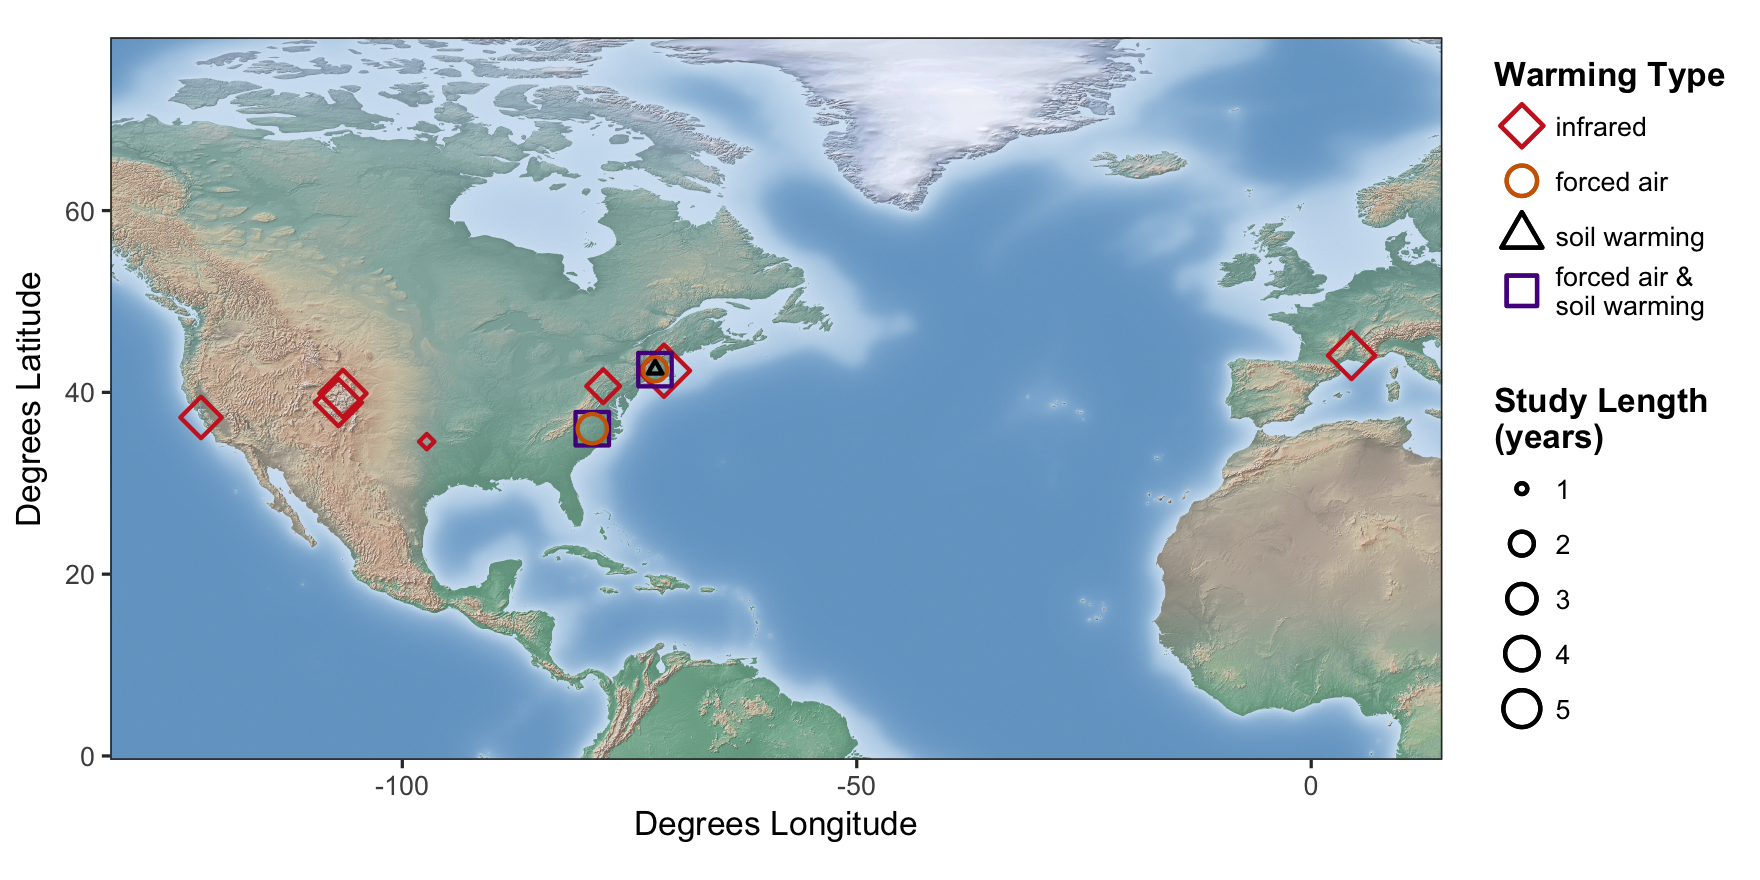
\includegraphics{/Users/aileneettinger/git/radcliffe/Analyses/maps/RadcliffeLocations_Experiments_Open.png} 
\caption{\textbf{Climate data from 12 climate change experiments in North America and Europe are included in the C3E database and analyzed here.} See Supplemental Materials, Tables S1 and S2 for details.} 
 \label{fig:map}
 \end{figure}
\clearpage
\begin{figure}[h]
\centering
 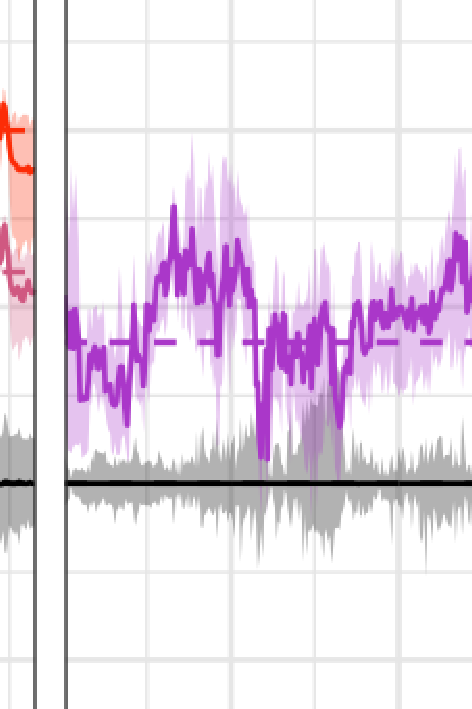
\includegraphics{/Users/aileneettinger/git/radcliffe/Analyses/figures/WarmingEffects_TimeSeries_SoilTemp1Mean_Deviation_NoPrecip.png}
 \caption{\textbf{Deviations in daily observed warming from mean soil temperature for 10 study sites.} Solid lines show observed difference between warming treatment (colors) and control (black) plots, averaged across replicates and years; shading shows 95\% confidence intervals. Dashed lines represent target warming levels. Two sites not shown here did not monitor soil temperature; we also excluded data from plots that manipulated precipitation. Mean annual temperature for experimental sites are shown in the upper right corner of each panel; panels are arranged by increasing annual temperature.} %The number of temperature treatment levels vary from one (e.g. exp08, exp11) to nine (exp07 and exp10, which used an unreplicated regression design). Daily temperature values were obtained by averaging across years for each day of the year in each temperature treatment in each study. 
 \label{fig:effwarm}
 \end{figure}
 \begin{figure}[p]
   \centering
 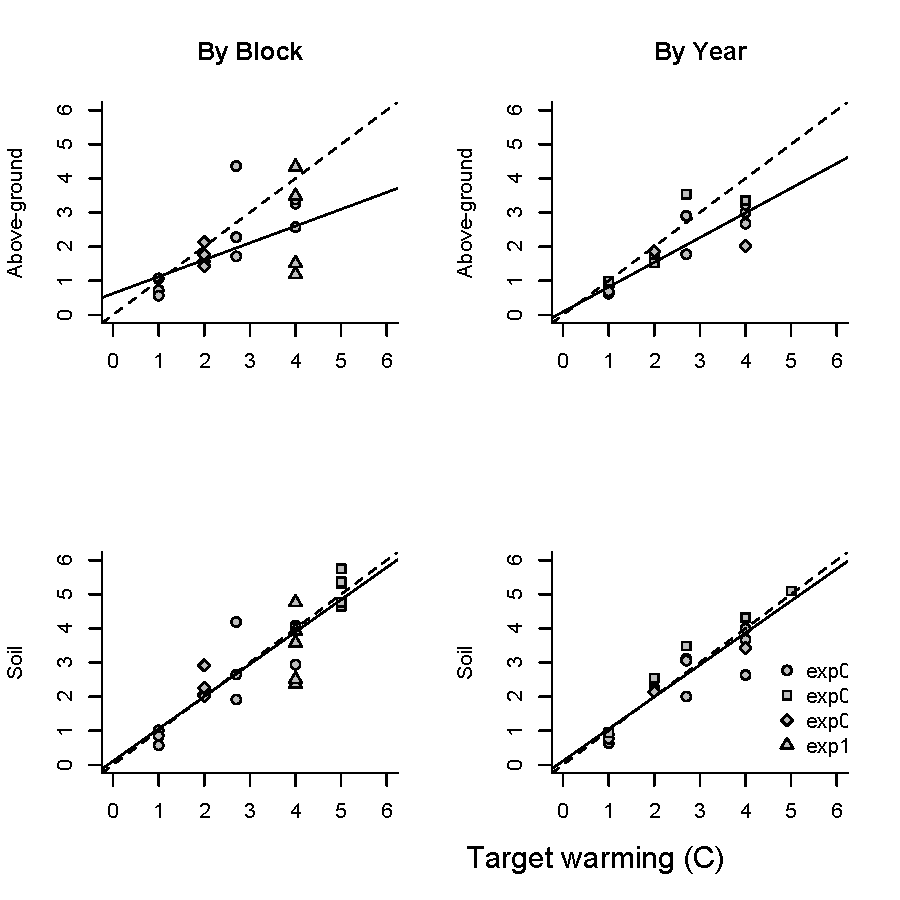
\includegraphics{/Users/aileneettinger/git/radcliffe/Analyses/figures/blockyearvar.pdf}  
 \caption{\textbf{Observed warming (i.e., the difference between treatment and control plots) over space and time, for above-ground and below-ground temperatures,} excluding data from plots that manipulated precipitation. The solid line is the fitted relationship between observed and target warming and the dashed line shows when observed warming is exactly equal to target warming (1:1). See Supplemental Materials (especially Tables S4 and S5) for details.}
 \label{fig:blockyear}
 \end{figure}
 
 \begin{figure}[p]
\centering
 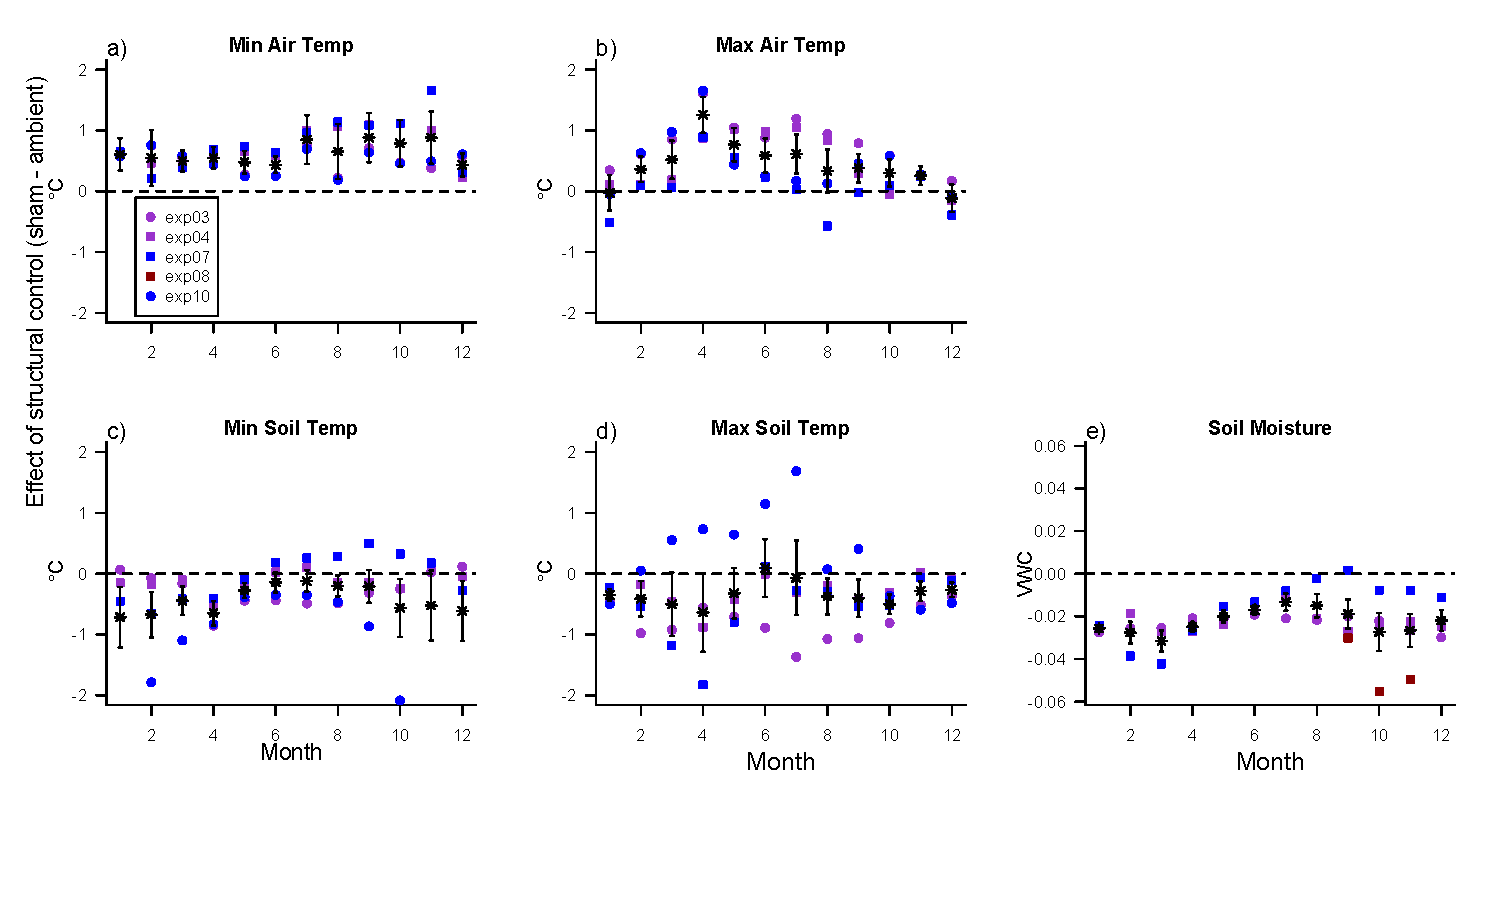
\includegraphics{/Users/aileneettinger/git/radcliffe/Analyses/figures/ShamVSAmbient_all.pdf}  
 \caption{\textbf{Deviations in measured abiotic variables by month in structural controls compared to ambient controls} (i.e., with no control chambers or warming infrastructure in place). Above-ground temperatures were higher, whereas below-ground temperature and soil moisture were lower in structural controls compared with ambient controls. We show overall (fixed) effects in black from monthly mixed-effects models; site-level random effects are shown by symbols in blue (for the three studies conducted at Harvard Forest in Massachusetts, USA) and pink (the two studies conducted at Duke Forest in North Carolina, USA).}
 \label{fig:shamamb}
 \end{figure}
\clearpage
 \begin{figure}[h]
    \centering
 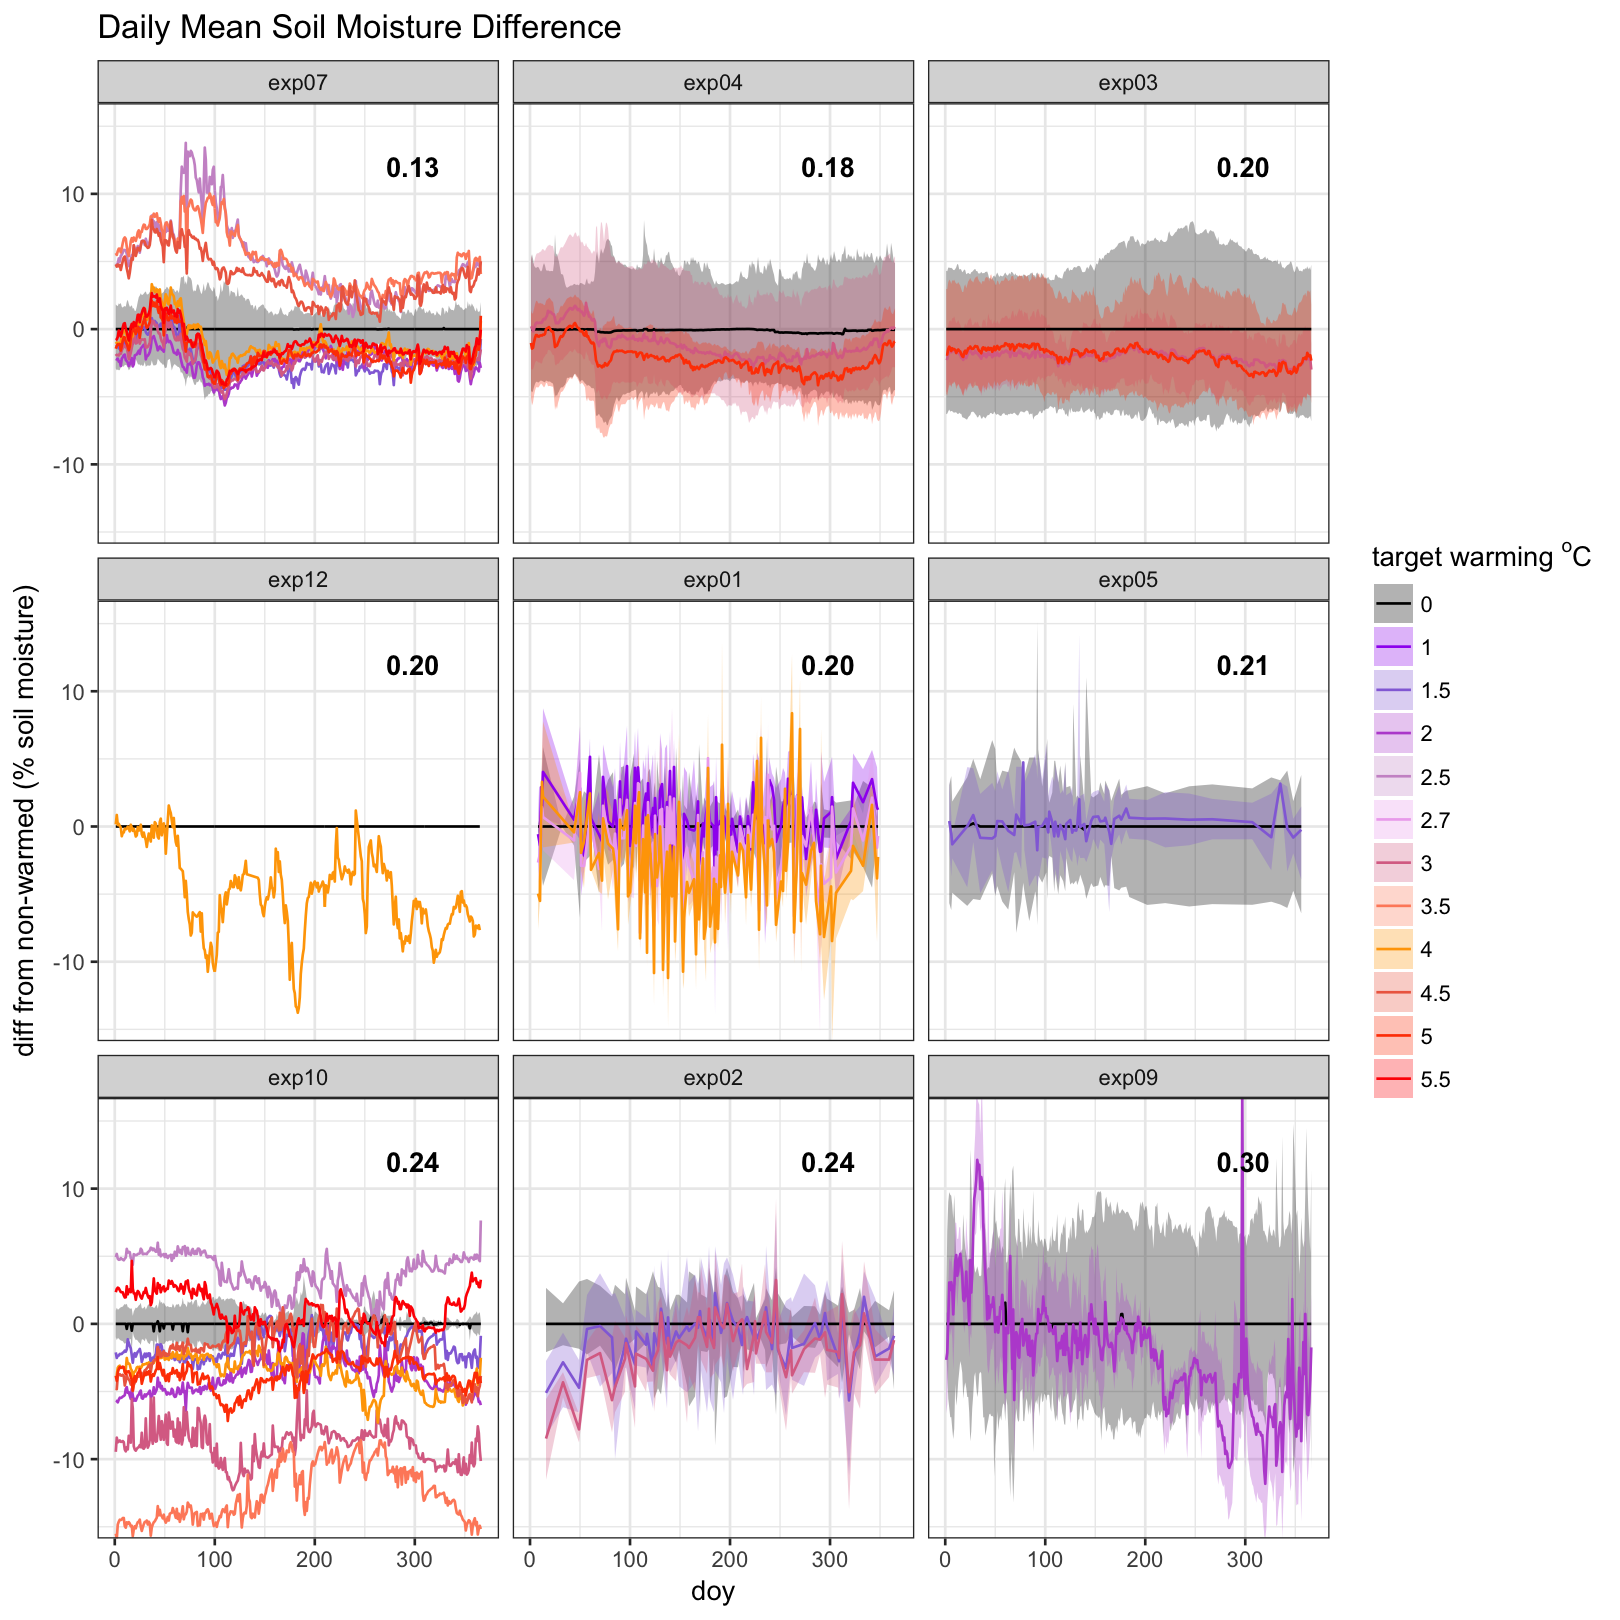
\includegraphics{/Users/aileneettinger/git/radcliffe/Analyses/figures/WarmingEffects_TimeSeries_SoilMoist_Deviation_NoPrecip.png}  
 \caption{\textbf{Deviations in daily observed soil moisture,} shown for the nine study sites that continuously monitored soil moisture, excluding data from plots that manipulated precipitation. Black lines represent control plots, and colored lines represent warming treatments with various target warming levels. The number of temperature treatment levels vary from one (e.g. exp08, exp11) to nine (exp07 and exp10, which used an unreplicated regression design). Mean annual soil moisture for the experimental site is shown in the upper right corner of each plot, and plots are arranged by increasing mean soil moisture. All experiments measured soil moisture in volumetric water content (VWC, as a proportion of the soil volume in the sample, scaled from 0 to 1).}. 
 \label{fig:mois}
 \end{figure}
 \begin{figure}[h]
 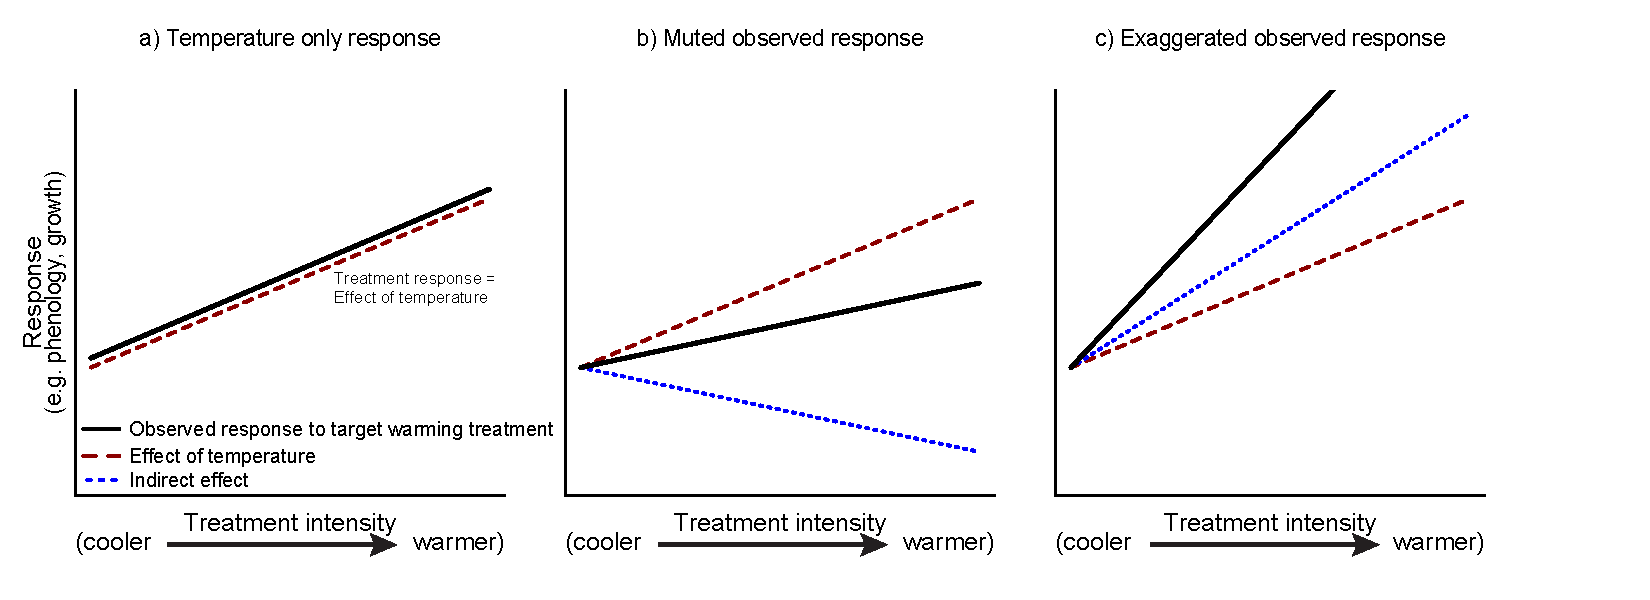
\includegraphics{/Users/aileneettinger/git/radcliffe/Analyses/figures/DirIndWarmingEffects.pdf} 
 \caption{\textbf{Possible biological responses to experimental climate change and their interpretation}. Direct responses to temperature alone (a) can be easily understood. Complications arise when biological responses are a mix of the direct and indirect effects of experimental warming. Then experimental warming may cause biological responses to be muted (b) or exaggerated (c). Slopes of these example lines assume a linear response with additive direct and indirect effects. The relationship between these effects could be more complex (e.g., nonlinear; antagonistic, multiplicative, or otherwise interactive).} 
\label{fig:biolimp}
  \end{figure}
%%%%%%%%%%%%%%%%%%%%%%%%%%%%%%%%%%%%%%%%
\end{document}
%%%%%%%%%%%%%%%%%%%%%%%%%%%%%%%%%%%%%%%%
